% !TEX root = ../my-thesis.tex
%
\chapter{Principles of magnetic confinement}
\label{sec:principles}

\section{Non-axisymmetric magnetic fields}
In a fusion device or plasma experiment, the motion of the particles and thus the deposition of particle and heat load on the plasma facing components is inextricably linked to the magnetic field topology. Therefore, a short overview over magnetic confinement based on \cite{Helander2014} will be given in this section.\\
For confinement of a plasma, a magnetic field is required, which is related to the plasma current \textbf{J} by Ampere's law
\begin{equation}
    \nabla \times \textbf{B} = \mu_0\textbf{J}.
\end{equation}
The magnetic force created by the plasma current balances the pressure force of the plasma and enables confinement. The amount of plasma current needed for confinement can be derived from the MHD equation of motion which results in
\begin{equation}
    \textbf{J} \times \textbf{B} = \nabla p \label{eq2}
\end{equation}
for the steady state case without flows. As a consequence, \textbf{J} and \textbf{B} lie in surfaces of constant pressure, i.e.
\begin{equation}
    \textbf{B}\cdot \nabla p =  \textbf{J}\cdot \nabla p = 0.
    \label{eq3}
\end{equation}
These surfaces have toroidal topology in a magnetically confined plasma.
Magnetic coordinates are used to describe these surfaces of constant pressure in a coordinate system where one coordinate is constant on these surfaces and the magnetic field lines are straight lines. Introducing the poloidal and toroidal angles $\vartheta$ and $\varphi$, a representation of the magnetic field as a composition of the toroidal and poloidal component is given by
\begin{equation}
    \textbf{B} = \nabla \psi \times \nabla \theta + \nabla \varphi \times \nabla \chi
\end{equation}
with $ \theta = \vartheta + \lambda$.\\
According to \ref{eq3}, $\psi$ and $\chi$ are constant on surfaces of constant pressure and can be chosen to vanish on the innermost surface of constant pressure, that is just a line and described as the magnetic axis. By calculating the surface integral, it can be easily shown that the magnetic flux through a poloidal cross section of constant $\varphi$ between the magnetic axis and a surface of constant $\psi$ is equal to $2\pi\psi$, while the poloidal magnetic flux through a surface of constant $\phi$ between the magnetic axis and a flux surface $\psi$ is equal to $2\pi\chi$. These surfaces of constant toroidal and poloidal flux are called flux surfaces. \\
$\chi$ can be interpreted as the derivative of $\psi$, which is called the rotational transform
\begin{equation}
    \iota = \frac{d\chi}{d\psi}
\end{equation}
and indicates the number of poloidal turns per toroidal turn of a field line, because $\theta$ and $\varphi$ vary in proportion along a field line:
\begin{equation}
    \frac{d\phi}{d\varphi} = \frac{\textbf{B}\cdot \nabla \phi}{\textbf{B}\cdot \nabla \varphi} = \frac{(\nabla \varphi \times \nabla \chi) \cdot \nabla \phi}{(\nabla \psi \times \nabla \theta) \cdot \nabla \varphi} = \iota
\end{equation}
Introducing $\alpha = \theta - \iota \varphi$ leads to the so called Clebsch representation of the magnetic field
\begin{equation}
    \textbf{B} = \nabla \psi \times \nabla \alpha,
\end{equation}
where $\textbf{B} \cdot \nabla \alpha = 0$ and $\alpha$ is constant along the magnetic field. Consequently, the magnetic field lines are straight in the $(\theta, \varphi)$-plane, which was one of the requirements for the magnetic coordinates. Thus, the magnetic field lines can be described by the two coordinates $\psi$ and $\alpha$. Because $\frac{d\theta}{d\varphi} = \iota$ along a field line , the poloidal angle of a field line changes by $2\pi \iota$ after one toroidal turn. If $\iota$ is a rational number, i.e. $\iota = \frac{n}{m}$, the field line returns to where it started, while it traces out the whole flux surface for irrational $\iota$. \\

Although the magnetic field in stellarators is mainly generated by the magnetic field coils, the plasma current \textbf{J} that is needed to balance the plasma pressure modifies the magnetic field and consists of parallel and perpendicular components
\begin{equation}
    \textbf{J} = \textbf{J}_{\parallel} + \textbf{J}_{\perp}.
\end{equation}
The perpendicular component is required to produce the magnetic force given in \ref{eq2} and the parallel component is needed to satisfy \ref{eq3}. Thus, the current is given by
\begin{equation}
    \textbf{J} = (u(\psi, \theta, \varphi)p'(\psi)+\frac{\langle \textbf{J}_{\parallel}\textbf{B}\rangle}{\langle \textbf{B}^2\rangle}) \textbf{B}+\frac{\textbf{B} \times \nabla p}{B^2}, \label{eq9}
\end{equation}
where $u(\psi, \theta, \varphi)$ satisfies the magnetic differential equation $\textbf{B}\cdot \nabla u = -(\textbf{B}\times \nabla \psi) \cdot \nabla (\frac{1}{B^2})$. The first and second term in \ref{eq9} describe the parallel current, where the first one is the so-called Pfirsch-Schlüter current and the second term the Ohmic current. The third term describes the perpendicular diamagnetic current. A more detailed derivation of the plasma currents is given in \cite{Chen2012}. \\
While the existence of MHD equilibria \cite{Moffatt1985} can be proven e.g. using the variational principle \cite{Helander2014}, the pressure profiles or field lines do not necessarily have to be continuous or the plasma current free from singularities. A Fourier expansion of the parallel current in equation \ref{eq9} reveals the possible singularities in the current on the rational surfaces, namely a surface current and a divergent Pfirsch-Schlüter current. While a detailed derivation of these singularities can be found in \cite{Helander2014}, we do not focus on the discussion of singularities in the current here as they can be avoided by giving up on the requirement of nested flux surfaces and allowing for magnetic islands at rational surfaces. \\
The representation used for the magnetic field here,
\begin{equation}
    \textbf{B} = \nabla \times \textbf{A} = \nabla \psi \times \nabla \theta + \nabla \varphi \times \nabla \chi, \label{eq10}
\end{equation}
is a general repsresentation of the magnetic field and does not necessarily require the existance of magnetic surfaces.  They exist if $\chi$ can be written as a representation of $\psi$, since then $\textbf{B} \cdot \nabla \psi = 0$, but are not generally required. According to equation \ref{eq10}, the field lines are Hamiltonian
\begin{equation}
    \frac{d\psi}{d\varphi} = \frac{\textbf{B} \cdot \nabla \psi}{\textbf{B} \cdot \nabla \varphi} = - \frac{\partial \chi}{\partial \theta}
\end{equation}
\begin{equation}
    \frac{d\theta}{d\varphi} = \frac{\textbf{B} \cdot \nabla \theta}{\textbf{B} \cdot \nabla \varphi} =  \frac{\partial \chi}{\partial \psi}
\end{equation}
and are generally chaotic. The Hamiltonian $\chi$ can be Fourier decomposed, leading to
\begin{equation}
    \chi (\psi, \theta, \varphi) = \chi_0 (\psi) + \sum_{m, n\neq 0} \chi_{m,n}(\psi)e^{i(m\theta-n\varphi)} := \chi_0 (\psi) + f(\psi, \theta, \varphi).
\end{equation}
If $\psi$ and $\alpha = \theta-\iota(\psi_0)\varphi$ are used as canonical coordinates, , the Hamiltonian can be replaced by
\begin{equation}
    H(\psi, \alpha, \varphi) = \chi(\psi, \theta, \varphi)-\iota(\psi_0)(\psi-\psi_0) = \chi_0(\psi) + f(\psi, \alpha) - \iota(\psi_0)(\psi-\psi_0),
\end{equation}
which is equal to
\begin{equation}
    H(\psi, \alpha, \varphi) = \frac{\chi_0''(\psi_0)(\psi- \psi_0)^2}{2}+f(\psi_0, \alpha).
\end{equation}
This Hamiltonian can be integrated and described the magnetic islands around the resonant surface. The shape of the islands depends on the potential $f(\psi_0, \alpha)$. if only the first term is kept in the Fourier expansion, the potential becomes sinusoidal and the system is equivalent to an ordinary pendulum with the island separatrix corresponding to $2\chi_{mn}$ and
\begin{equation}
    \psi-\psi_0 = \sqrt{\frac{4\chi_{mn}(1-cos(m\alpha))}{\iota'(\psi_0)}}.
\end{equation}
The width of the islands is
\begin{equation}
    \Delta \psi = \sqrt{\frac{32\chi_{mn}}{\iota'(\psi_0)}}.
\end{equation}
As magnetic fields without continous symmetry are in general chaotic, they do not have nested flux surfaces everywhere and chains of islands can form, which consist if nested flux surfaces on their own with their own rotational transform. \\
The existence and calculation of such nested flux surfaces is carried out by the VMEC code based on the variational principle \cite{Hirshman1983},\cite{Hirshman1986}.

\section{VMEC principles}

\section{Magnetic field in Wendelstein 7-X}
In the stellarator experiment Wendelstein 7-X \cite{Beidler1990},\cite{Klinger2013}, the magnetic field has been optimized for good MHD-stability and good neoclassical confinement \cite{Grieger1992}. It is the first device of the HELIAS line \cite{Nuhrenberg1986}, in which the plasma currents, i.e. the bootstrap current, the Pfirsch-Schlüter current and the diamagnetic current and their effects on the magnetic field are minimized \cite{Dinklage2018}.\\
The main magnetic field in Wendelstein 7-X is generated by 50 non-planar and 20 planar superconducting magnetic field coils that are cooled with liquid helium \cite{Rummel2012}. According to the five-fold symmetry of Wendelstein 7-X, there exist five different types of non-planar and two types of planar magnetic field coils made of NbTi, which are installed in each of the ten half modules of the stellarator. The flip-symmetric installation of two half modules results in the five identical modules composing Wendelstein 7-X. \\
The magnetic field generated by the coils and plasma currents determines the heat and particle load onto the plasma facing components, which are controlled by a chain of magnetic islands at the edge of the plasma. The number of islands depends on the edge rotational transform and is shown in figure \ref{fig:1} for the standard configuration, where an edge $\iota$ of 5/5 creates five islands.
\begin{figure}[!htb]
    \centering
    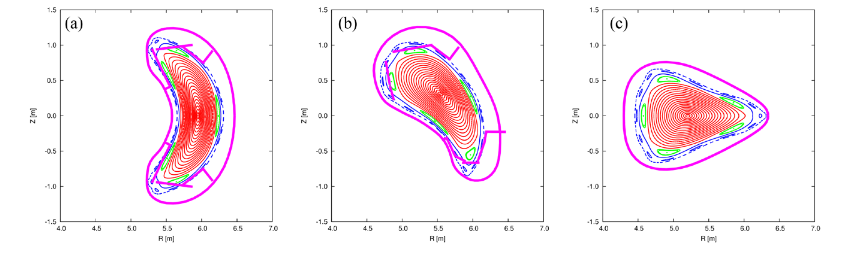
\includegraphics[width=\textwidth]{images/islands.png}
    \caption{Poincaré plots of the vacuum magnetic field in standard configuration for three different poloidal cross sections from \cite{Suzuki2016}. The islands intersecting the plasma facing components are shown in green, the target plates in pink.} \label{fig:1}
\end{figure}

The rotational transform can be varied between edge $\iota$ = 5/6 in the so-called low-iota configuration and edge $\iota$ = 4/5 in the high-iota configuration, with six and four magnetic islands respectively \cite{Knieps2021}. Following the island divertor concept \cite{Konig2002}, \cite{Renner2002}, target plates made of graphite intersect the islands to divert the heat and particle load and are shown in figure \ref{fig:1}.


\section{Heat load on the plasma facing components}

The heat load on the plasma facing components that intersect the islands is limited by the material properties of the plasma facing components and therefore needs to be monitored closely. While the divertor targets are designed for a heat flux of up to 10\,MW/m$^2$, significantly lower heat loads of 0.5\,MW/m$^2$ can be tolerated on the surrounding baffle structures \cite{Jakubowski2018}. Therefore, the surface temperature of the divertor targets and the surrounding structures are monitored closely by a set of infrared diagnostics to avoid overloading of the components and to study the particle and heat load deposition pattern on the plasma facing components. Based on the tenperature of the components, the heat flux can be derived using the two-dimensional thermal model THEODOR \cite{Sieglin2015}.
\begin{figure}[!htb]
    \centering
    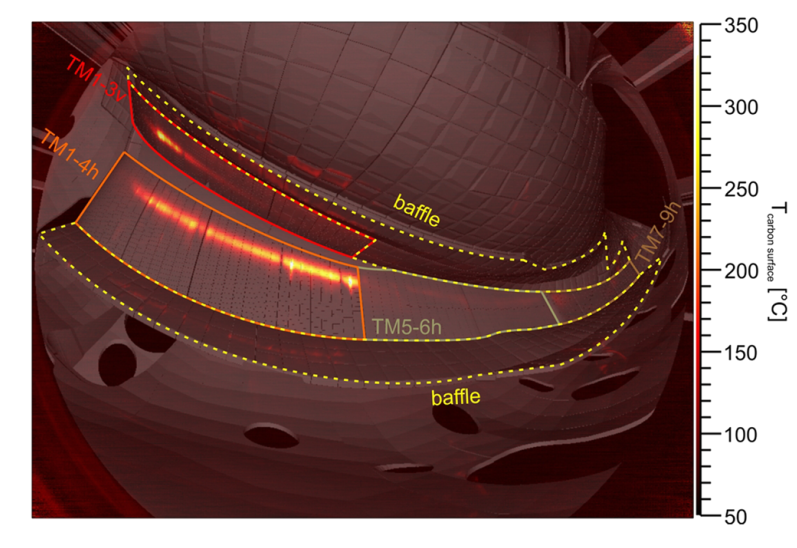
\includegraphics[scale = 0.5]{images/ir_image.png}
    \caption{Infrared image of one divertor module and the surrounding plasma facing components overlaid with a CAD model, from \cite{Jakubowski2018}} \label{fig:2}
\end{figure}
During the last experimental campaign, nine out of the ten divertor modules in Wendelstein 7-X - a lower and an upper divertor unit in each of the five modules of the torus - have been monitored by a set of different infrared and visible cameras. Infrared microbolometric cameras, which have been specifically designed to work in a magnetic field of up to 3\,T use a fish eye lens to provide a wide angle view of the whole divertor units. Detailed specifications of the cameras in use are given in \cite{Jakubowski2018}. The cameras provide a spectral response in the range of 8-10\,$\mu$m and can therefore be used to measure surface temperatures between 30 and 5000$^\circ$C. An example for the temperature distribution measured in one divertor unit is given in figure \ref{fig:2}, where the temperature distribution is overlaid by a CAD-model of the plasma facing components. This representation allows for a detailed sudy of the heat load deposition pattern on the plasma facing components \cite{Niemann2020} as well as the localization of individual thermal hotspots depending on the magnetic field configuration and the location of the magnetic islands.

% ToDo: Add some details about the coil configuration here

\begin{figure}[!htb]
    \centering
    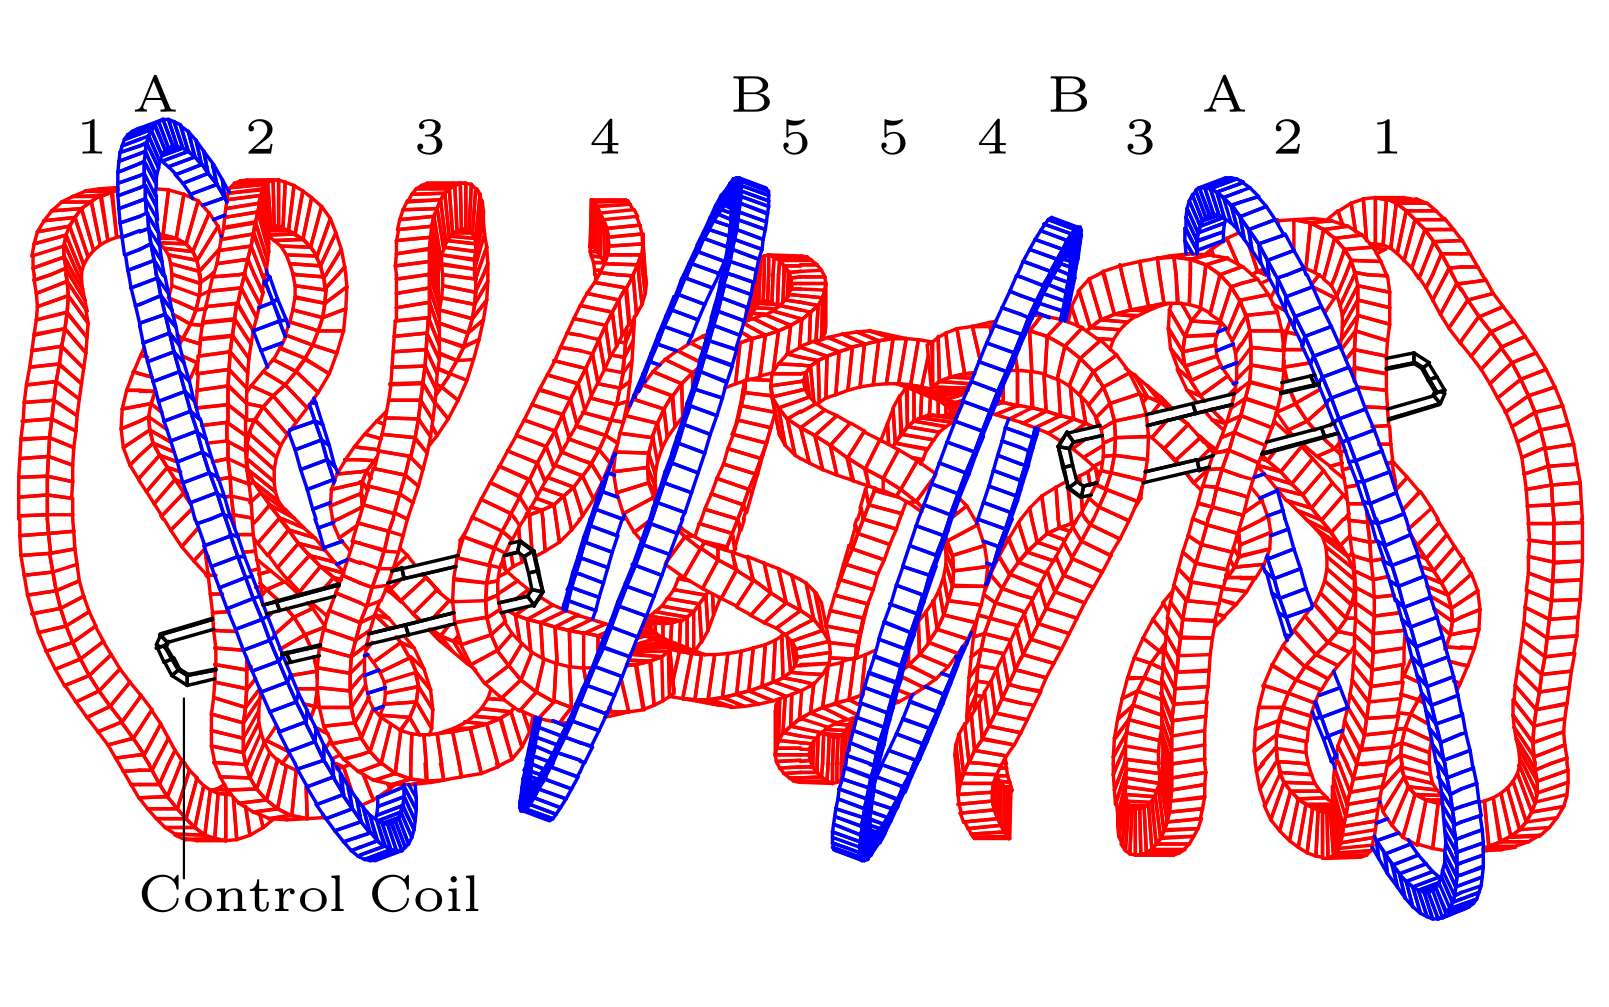
\includegraphics[scale = 0.7]{images/magnetic-coils.png}
    \caption{Coil diagram from one of the five W7X modules. The red coils are the non-planar coils. The blue coils are the two planar coils, $A$ and $B$. Taken from \ref{Böckenhoff_2018}} \label{fig:3}
\end{figure}